\documentclass[border=4pt]{standalone}
\usepackage{tikz}
\usetikzlibrary{arrows.meta, positioning, shadows.blur}
\begin{document}
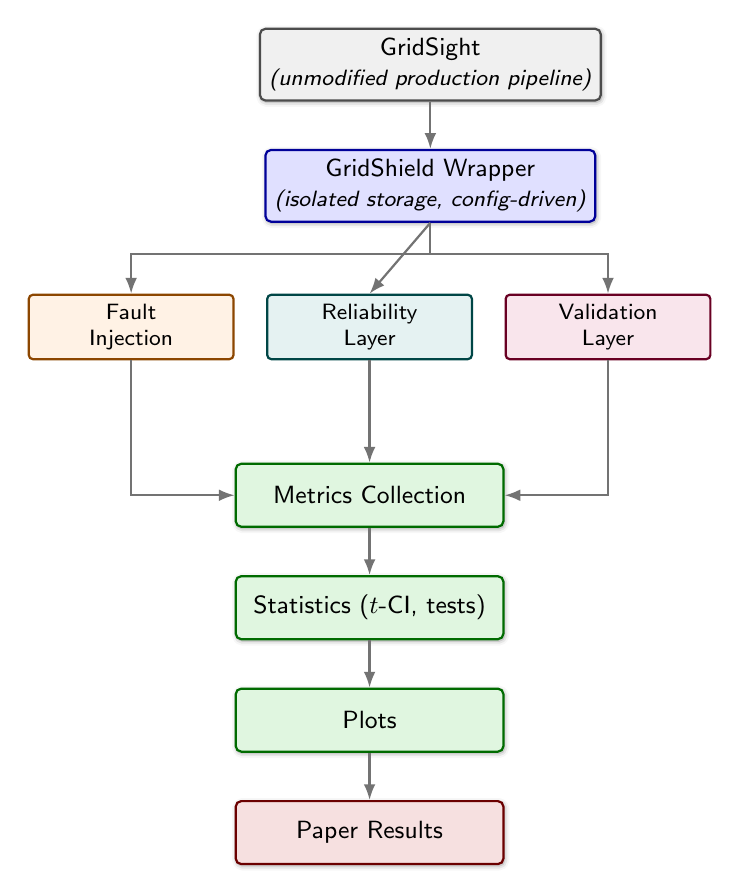
\begin{tikzpicture}[
  node distance=6mm and 6mm,
  box/.style={rectangle, rounded corners=2pt, draw=#1!60!black, fill=#1!12,
              minimum width=34mm, minimum height=8mm, align=center,
              font=\sffamily\small, thick, blur shadow={shadow blur steps=3,shadow xshift=0.4pt,shadow yshift=-0.6pt}},
  sub/.style={rectangle, rounded corners=1.5pt, draw=#1!55!black, fill=#1!10,
              minimum width=26mm, minimum height=6.5mm, align=center,
              font=\sffamily\footnotesize, thick},
  arr/.style={-{Latex[length=2mm,width=1.5mm]}, thick, draw=black!55}
]

\node[box=gray] (gridsight) {GridSight\\\footnotesize\textit{(unmodified production pipeline)}};
\node[box=blue, below=of gridsight] (wrapper) {GridShield Wrapper\\\footnotesize\textit{(isolated storage, config-driven)}};

\node[sub=orange, below=9mm of wrapper, xshift=-38mm] (fault) {Fault\\Injection};
\node[sub=teal, right=4mm of fault] (reliab) {Reliability\\Layer};
\node[sub=purple, right=4mm of reliab] (valid) {Validation\\Layer};

\node[box=green!70!black, below=13mm of reliab] (metrics) {Metrics Collection};
\node[box=green!70!black, below=of metrics] (stats) {Statistics ($t$-CI, tests)};
\node[box=green!70!black, below=of stats] (plots) {Plots};
\node[box=red!70!black, below=of plots] (paper) {Paper Results};

\draw[arr] (gridsight) -- (wrapper);
\draw[arr] (wrapper.south) -- ++(0,-4mm) -| (fault.north);
\draw[arr] (wrapper.south) -- (reliab.north);
\draw[arr] (wrapper.south) -- ++(0,-4mm) -| (valid.north);
\draw[arr] (fault.south) |- (metrics.west);
\draw[arr] (reliab) -- (metrics);
\draw[arr] (valid.south) |- (metrics.east);
\draw[arr] (metrics) -- (stats);
\draw[arr] (stats) -- (plots);
\draw[arr] (plots) -- (paper);

\end{tikzpicture}
\end{document}
